\newpage
\appendix
\section{Datalog Background}
\label{app:datalog}

The Datalog language is defined over relational tables; it is a purely logical query language that makes no changes to the stored tables. A Datalog {\em program} is a set of {\em rules} or named queries, in the spirit of SQL's {\em view}s.  A simple Datalog rule has the form:
\[
	r_{\mbox{\em head}}(\langle\mbox{\em col-list}\rangle) \mbox{{ \tt :- }} r_1(\langle\mbox{{\em col-list}}\rangle), \ldots, r_n(\langle\mbox{{\em col-list}}\rangle)
\]
Each term $r_i$ represents a relation, either stored (a database
table) or derived (the result of other rules).  Relations' columns are
listed as a comma-separated list of variable names; by convention,
variables begin with capital letters.  Terms to the right of the {\tt
  :-} symbol form the rule {\em body} (corresponding to the {\tt
  \small FROM} and {\tt \small WHERE} clauses in SQL), the relation to
the left is called the {\em head} (corresponding to the {\tt \small
  SELECT} clause in SQL).  Each rule is a logical assertion that the
head relation contains those tuples that can be generated from the
body relations.  Tables in the body are {\em unified} (joined
together) based on the positions of the repeated variables in the
column lists of the body terms.  For example, a canonical Datalog
program for recursively computing paths from links~\cite{loo-sigmod06}
is shown in Figure~\ref{fig:datalogsql} (ignoring the Overlog-specific
{\tt @} notation), along with analogous SQL for the inductive rule.
Note how the SQL {\tt \small WHERE} clause corresponds to the repeated
use of the variable {\tt \small To} in the Datalog.

%\rcs{START} Overlog extends Datalog with distribution and a semantics for table updates.
%\rcs{END Between START, END isn't really true in \JOL, and is (I
%think) a confusing way to think about location specifiers.  For one
%thing, \JOL doesn't partition the tables, because it doesn't
%understand membership.  Also, \JOL supports local tables, and
%networks that contain multiple programs.  Recommend next paragraph
%instead.}
\begin{figure}[t]
%\begin{minipage}{0.5\linewidth}
\begin{small}
\begin{verbatim}
path(@From, To, To, Cost) 
        :- link(@From, To, Cost);
path(@From, End, To, Cost1+Cost2)
        :- link(@From, To, Cost1),
           path(@To, End, NextHop, Cost2);
\end{verbatim}
\end{small}
%\end{minipage}
%\begin{minipage}{0.5\linewidth}
\begin{small}
\begin{verbatim}
	WITH path(Start, End, NextHop, Cost) AS
	  ( SELECT link.From, path.End, 
	           link.To, link.Cost+path.Cost
	      FROM link, path
	     WHERE link.To = path.Start );
\end{verbatim}
\end{small}
%\end{minipage}
\vspace{-12pt}
\caption{Example Overlog for computing paths from links, along with an SQL translation of the second rule.}
\label{fig:datalogsql}
\end{figure}

\begin{figure}[t]
\centering
\begin{small}
\begin{verbatim}
// fqpath: Fully-qualified paths.
// Base case: root directory has null parent
fqpath(Path, FileId) :-
    file(FileId, FParentId, _, true),
    FParentId = null, Path = "/";

fqpath(Path, FileId) :-
    file(FileId, FParentId, FName, _),
    fqpath(ParentPath, FParentId),
    // Do not add extra slash if parent is root dir
    PathSep = (ParentPath = "/" ? "" : "/"),
    Path = ParentPath + PathSep + FName;
\end{verbatim}
\end{small}
\vspace{-12pt}
\caption{Example Overlog for computing fully-qualified pathnames from
  the base file system metadata in \BOOM-FS.}
\label{fig:bfs-path}
\vspace{-12pt}
\end{figure}

\section{Validation of Initial Prototype}
\label{app:experiment}
\begin{figure*}[t]
\begin{minipage}{0.5\linewidth}
        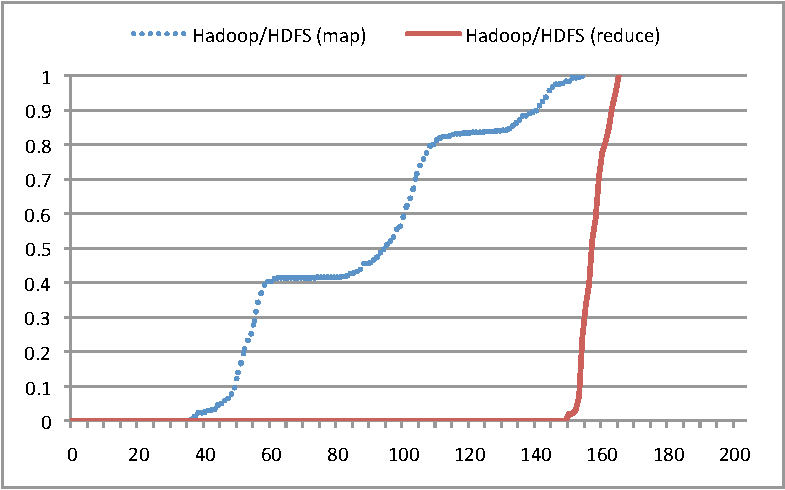
\includegraphics[width=0.95\linewidth]{graphs/hadoop_hdfs}
\end{minipage}
\begin{minipage}{0.5\linewidth}
        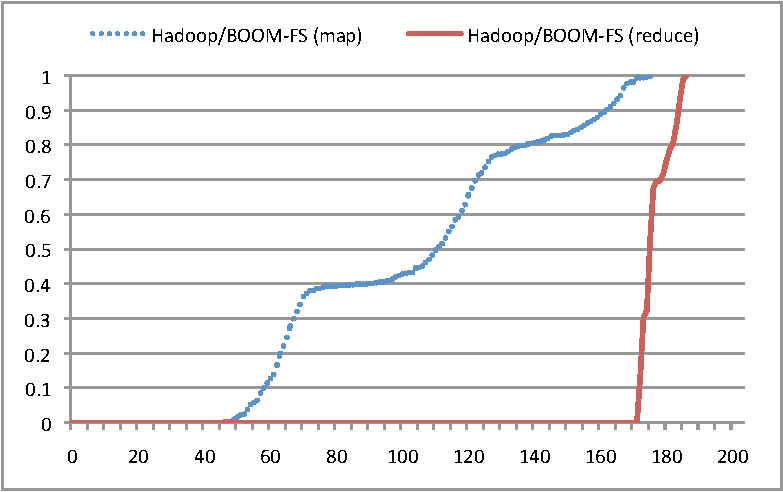
\includegraphics[width=0.95\linewidth]{graphs/hadoop_bfs}
\end{minipage}
\begin{minipage}{0.5\linewidth}
        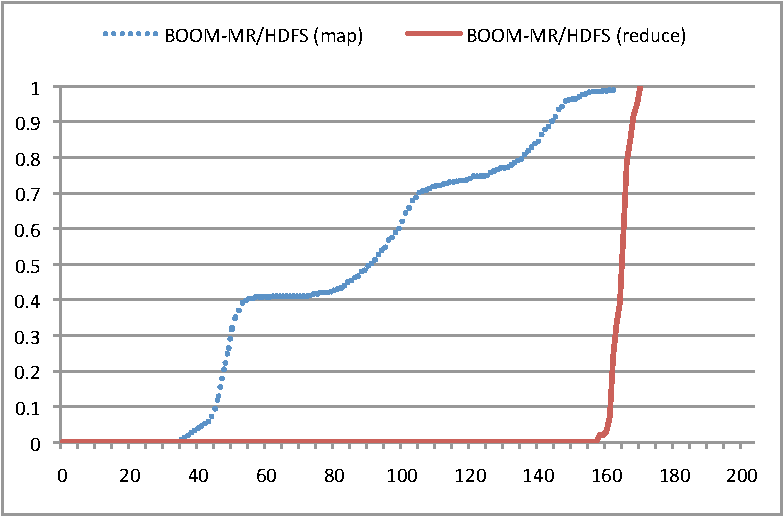
\includegraphics[width=0.95\linewidth]{graphs/bmr_hdfs}
\end{minipage}
\begin{minipage}{0.5\linewidth}
        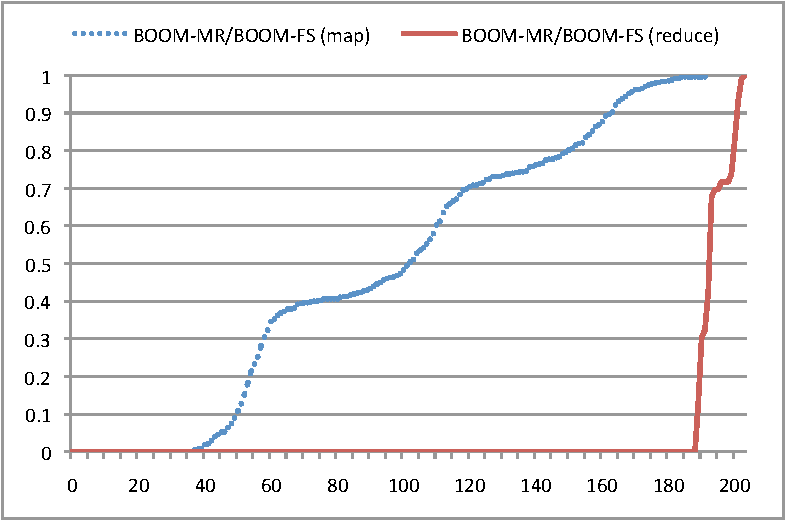
\includegraphics[width=0.95\linewidth]{graphs/bmr_bfs}
\end{minipage}
\caption{CDF of map and reduce task completion for Hadoop and \BOOM-MR
  over HDFS and \BOOM-FS.  In all graphs, the horizontal axis is
  elapsed time in seconds, and the vertical represents \% of tasks completed.}
\label{fig:ec2experiment}
\vspace{-10pt}
\end{figure*}

While improved performance was not a goal of our work, we wanted to
ensure that the performance of \BOOMA was competitive with Hadoop. To
that end, we conducted a series of performance experiments using a
101-node cluster on Amazon EC2. One node executed the Hadoop \JT\ and
the DFS \NN, while the remaining 100 nodes served as slaves for
running the Hadoop {\TT}s and DFS {\DN}s. The master node ran on an
``high-CPU extra large'' EC2 instance with 7.2 GB of memory and 8
virtual cores. Our slave nodes executed on ``high-CPU medium'' EC2
instances with 1.7 GB of memory and 2 virtual cores. Each virtual core
is the equivalent of a 2007-era 2.5Ghz Intel Xeon processor.

For our experiments, we compared \BOOMA with Hadoop 18.1. Our workload
was a wordcount job on a 30 GB file. The wordcount job consisted of
$481$ map tasks and $100$ reduce tasks. Each of the $100$ slave nodes
hosted a single \TT instance that can support the simultaneous
execution of $2$ map tasks and $2$ reduce tasks.

Figure~\ref{fig:ec2experiment} contains four performance graphs,
comparing the performance of different combinations of Hadoop
MapReduce, HDFS, \BOOM-MR, and \BOOM-FS. Each graph reports a
cumulative distribution of map and reduce task completion times (in
seconds).  The map tasks complete in three distinct ``waves''. This is
because only $2\times100$ map tasks can be scheduled at once. Although
all $100$ reduce tasks can be scheduled immediately, no reduce task
can finish until all maps have been completed, because each reduce
task requires the output of all map tasks.

The upper-left graph describes the performance of Hadoop running on
top of HDFS, and hence serves as a baseline for the subsequent
graphs. The lower-left graph details \BOOM-MR running over HDFS. This
graph shows that map and reduce task completion times under \BOOM-MR
are nearly identical to Hadoop 18.1. The upper-right and lower-right
graphs detail the performance of Hadoop MapReduce and \BOOM-MR running
on top of \BOOM-FS, respectively. \BOOM-FS performance is slightly
worse than HDFS, but remains very competitive.

\section{MapReduce Scheduling}
\label{sec:scheduling}
MapReduce scheduling has been the subject of recent research, and one
of our early motivations for building \BOOMA was to make that research
extremely easy to carry out. In our initial \BOOM-MR prototype, we
implemented Hadoop's default First-Come-First-Served policy for task
scheduling, which was captured in 9 rules (96 lines) of scheduler
policy. Next, we implemented the recently-proposed LATE
policy~\cite{late-sched} to evaluate both (a) the difficulty of
prototyping a new policy, and (b) the faithfulness of our
Overlog-based execution to that of Hadoop using two separate
scheduling algorithms.

The LATE policy presents an alternative scheme for speculative task
execution on {\em straggler} tasks~\cite{late-sched}, in an effort to
improve on Hadoop's policy.  There are two aspects to each policy:
choosing which tasks to speculatively re-execute, and choosing {\TT}s
to run those tasks.  Original Hadoop re-executes a task if its
progress is more than 0.2 (on a scale of $[0..1]$) below the mean
progress of similar tasks; it assigns speculative tasks using the same
policy as it uses for initial tasks. LATE chooses tasks to re-execute
via an {\em estimated finish time} metric based on the task's
\emph{progress rate}. Moreover, it avoids assigning speculative tasks
to {\TT}s that exhibit slow performance executing similar tasks, in
hopes of preventing the creation of new stragglers.

The LATE policy is specified in the paper via just three lines of
pseudocode, which make use of three performance statistics called {\em
  SlowNodeThreshold}, {\em SlowTaskThreshold}, and {\em
  SpeculativeCap}.  The first two of these statistics correspond to
the 25th percentiles of progress rates across {\TT}s and across tasks,
respectively.  The {\em SpeculativeCap} is suggested to be set at 10\%
of available task slots~\cite{late-sched}.  We compute these
thresholds via the five Overlog rules shown in
Figure~\ref{fig:latePolicy}.  Integrating the rules into \BOOM-MR
required modifying two additional Overlog rules that identify tasks to
speculatively re-execute, and that choose {\TT}s for scheduling those
tasks.

% If a \TT asks for new a new task and there are fewer than {\em SpeculativeCap} speculative tasks running:
% \begin{enumerate}
% \item Ignore the request if the \TT progress for running tasks is below some {\em SlowNodeThreshold}
% \item Rank current running tasks by the estimated finish time
% \item Launch a copy of the highest-ranked task with progress rate below {\em SlowTaskThreshold}
% \end{enumerate}

%The primary inputs to the LATE policy are the {\em SpeculativeCap}, {\em SlowTaskThreshold} and the {\em SlowNodeThreshold} values, which provide thresholds for pruning tasks and nodes from consideration. The SpeculativeCap is a single system level query maintained in the scheduler.olg module, and is used to limit the total number of speculative map and reduce tasks. SlowTaskThreshold and SlowNodeThreshold values are categorized by the job identifier and task type (map or reduce). Selecting which tasks to speculate, and on which trackers they should execute, required changes to two queries in the first-come first-serve policy.olg module and the additional 6 queries. %shown in  Figure~\ref{fig:latePolicy}. 

%A task is only considered for speculation if its progress rate falls below the SlowTaskThreshold in its given category.  Queries L1 - L3 maintain this threshold value for each category. Query L1 determines the progress rate for a given task based on its current progress and running time. Query L2 forms a list of the progress rates for each task category. Finally, query L3 computes a SlowTaskThreshold for each task type of a job by taking the lower 25th percentile of the progress rate list. 
%The LATE policy ensures that speculative tasks execute on ``fast'' nodes by pruning \TT nodes whose rate of progress for a given task category fall below some threshold. Queries L4 - L6 maintain this threshold value for each task category. The first query L4, computes the average progress that a given \TT has made for each task category and stores that result in the taskPR table. Query L5 forms a list of the average progress rates out of each category by aggregating over the taskPR table, and the result of this query is stored in the trackerPRList table. Query L6 computes the slowNodeThreshold for each category by taking the 25th percentile of the list of rates stored in the trackerPRList table.


% \jmh{Tyson/Khaled to write one paragraph here on the size/complexity of the LATE implementation.}
% 
% \jmh{Tyson/Khaled to write on paragraph here with motivation for
% affinity scheduler here, a sketch of the policy that was
% implemented.}

% \subsection{LATE Evaluation}
Figure~\ref{fig:ec2reduce} shows the cumulative distribution of the
completion time for reduce task executions on EC2 under normal load,
and with artificial extra load placed on six straggler nodes.  The
same wordcount workload was used for this experiment but the number of
reduce tasks was increased from $100$ to $400$ in order to produce two
waves of reduce tasks.  The plots labeled ``No Stragglers'' represent
normal load.  The plots labeled ``Stragglers'' and ``Stragglers
(LATE)'' are taken under the (six node) artificial load using the
vanilla Hadoop and LATE policies (respectively) to identify
speculative tasks.  We do not show a CDF of the map task execution
time since the artificial load barely affects it --- the six
stragglers have no effect on other map tasks, they just result in a
slower growth from just below $100\%$ to completion.
%Figure~\ref{fig:ec2map} shows that the delay due to the loaded map stragglers only
%affects those six nodes.  
The first wave of $200$ reduce tasks is scheduled concurrently with
all the map tasks. This first wave of reduce tasks will not finish
until all map tasks have completed, which increases the completion time
of these tasks as indicated in the right portion of the graph. The
second wave of $200$ reduce tasks will not experience the delay due to
unfinished map work since it is scheduled after all map tasks have
finished. These shorter completion times are reported in the left
portion of the graph. Furthermore, stragglers have less of an impact
on the second wave of reduce tasks since less work (i.e., no map work)
is being performed. Figure~\ref{fig:ec2reduce} shows this effect, and
also demonstrates how the LATE implementation in \BOOMA handles
stragglers much more effectively than the default speculation policy
ported from Hadoop.  This echoes the results of Zaharia et
al.~\cite{late-sched}

\begin{figure}[tb]
  \centering
  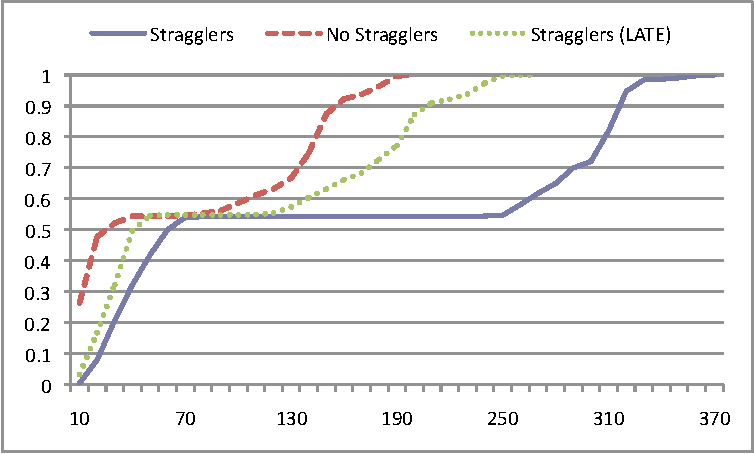
\includegraphics[width=0.95\linewidth]{graphs/reduce_stragglers}
  \caption{CDF of reduce task completion times (secs), with and without stragglers.}
  \label{fig:ec2reduce}
  \vspace{-12pt}
\end{figure}

\section{Validation: High Availability}
\label{sec:relyeval}

\begin{figure}[t]
  \centering
  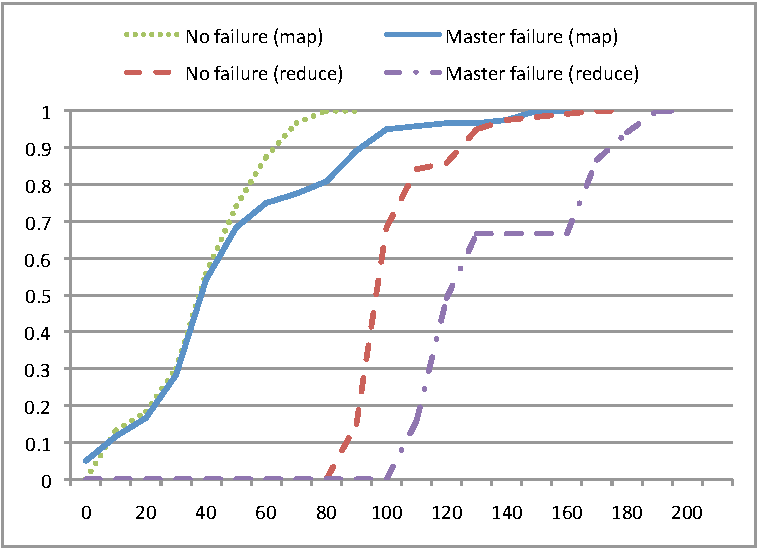
\includegraphics[width=0.95\linewidth]{graphs/failover}
  \caption{CDF of completed tasks over time (secs), with and without
    primary master failure.}
  \label{fig:failover}
\end{figure}

After adding support for high availability to the \BOOM-FS \NN
(Section~\ref{sec:rely}), we wanted to evaluate two properties of our
implementation. At a fine-grained level, we wanted to ensure that our
complete Paxos implementation was operating according to the
specifications in the literature.  This required logging and analyzing
network messages sent during the Paxos protocol. This was a natural
fit for the metaprogrammed tracing tools we discussed in
Section~\ref{sec:monitor}. We created unit tests to trace the message
complexity of our Paxos code, both at steady state and under
churn. When the message complexity of our implementation matched the
specification, we had more confidence in the correctness of our code.

Second, we wanted to see the availability feature ``in action'', and
to get a sense of how our implementation would perform in the face of
master failures. Specifically, we evaluated the impact of the
consensus protocol on \BOOMA system performance, and the effect of
failures on overall completion time. We ran a Hadoop wordcount job on
a 5GB input file with a cluster of 20 EC2 nodes, varying the number of
master nodes and the failure condition.  These results are summarized
in Table~\ref{tab:rely}. We then used the same workload to perform a
set of simple fault-injection experiments to measure the effect of
primary master failures on job completion rates at a finer grain,
observing the progress of the map and reduce jobs involved in the
wordcount program. Figure~\ref{fig:failover} shows the cumulative
distribution of the percentage of completed map and reduce jobs over
time, in normal operation and with a failure of the primary \NN during
the map phase.  Note that Map tasks read from HDFS and write to local
files, whereas Reduce tasks read from Mappers and write to HDFS.  This
explains why the CDF for Reduce tasks under failure goes so crisply flat in
Figure~\ref{fig:failover}: while failover is underway after an HDFS
\NN failure, some nearly-finished Map tasks may be able to complete,
but no Reduce task can complete.

\begin{table}
	\begin{center}
		\scriptsize{
\begin{tabular}{|c|c|r|r|}
\hline
Number of & Failure   & Avg. Completion & Standard \\ 
{\NN}s    & Condition & Time (secs)      & Deviation\\ \hline
1 & None & 101.89 & 12.12 \\ \hline
3 & None & 102.70 & 9.53 \\ \hline
3 & Backup & 100.10 & 9.94 \\ \hline
3 & Primary & 148.47 & 13.94 \\
\hline
\end{tabular}
}
\end{center}
%\vspace{-12pt}
\caption{Job completion times with a single \NN, 3 Paxos-enabled {\NN}s, backup \NN failure, and primary \NN failure.}
\label{tab:rely}
\end{table}

\begin{figure}[p]
%\begin{minipage}{0.5\linewidth}
\begin{small}
\begin{verbatim}
// Compute progress rate per task
taskPR(JobId, TaskId, Type, ProgressRate) :- 
    task(JobId, TaskId, Type, _, _, _, Status), 
    Status.state() != FAILED,  
    Time = Status.finish() > 0 ?
        Status.finish() : currentTimeMillis(), 
    ProgressRate = Status.progress() / 
                    (Time - Status.start()); 
\end{verbatim}
\end{small}
\begin{small}
\begin{verbatim}
// For each job, compute 25th pctile rate across tasks
taskPRList(JobId, Type, percentile<0.25, PRate>) :- 
    taskPR(JobId, TaskId, Type, PRate); 
\end{verbatim}
\end{small}
\begin{small}
\begin{verbatim}
// Compute progress rate per tracker
trackerPR(Tracker, JobId, Type, avg<PRate>) :- 
    task(JobId, TaskId, Type, _), 
    taskAttempt(JobId, TaskId, _, Progress, State, 
                Phase, Tracker, Start, Finish), 
    State != FAILED, 
    Time = Finish > 0 ? Finish : currentTimeMillis(), 
    PRate = Progress / (Time - Start);  
\end{verbatim}
\end{small}
\begin{small}
\begin{verbatim}
// For each job, compute 25th pctile rate across trackers
trackerPRList(JobId, Type, percentile<0.25, AvgPRate>) :- 
    trackerPR(_, JobId, Type, AvgPRate); 
\end{verbatim}
\end{small}
\begin{small}
\begin{verbatim}
// Compute available map/reduce slots
speculativeCap(sum<MapSlots>, sum<ReduceSlots>) :-
    taskTracker(_, _, _, _, _, _,  
                MapCount, ReduceCount,
                MaxMap, MaxReduce),
    MapSlots = MaxMap - MapCount,
    ReduceSlots = MaxReduce - ReduceCount;
\end{verbatim}
\end{small}
%\end{minipage}
\vspace{-12pt}
\caption{Overlog to compute statistics for LATE.}
\label{fig:latePolicy}
\end{figure}
